% Appendix B
 
\chapter{Designing Figures}

This section contains recommendations on designing effective figures. We will cover graphs as well as diagrams.

We compiled the material in this appendix from the following sources:
\begin{itemize}
  \item the book ``Designing Science Presentations: A Visual Guide to Figures, Papers, Slides, Posters, and More'' \cite{Carter12},
  \item the book ``Information Visualization: Perception for Design'' \cite{Ware12}, and 
  \item …
\end{itemize}

\section{Fundamental Concepts}

\subsection{Gestalt Laws}

The Gestalt laws have been known since the early 1900s. They describe how we perceive patterns. In the following, we will discuss the following Gestalt laws: proximity, similarity, connectedness, continuity, symmetry, closure, and relative size.

\begin{marginfigure}
\centering
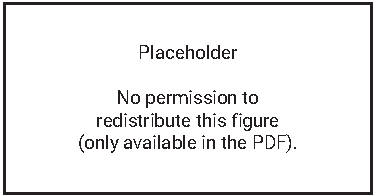
\includegraphics[width=1\textwidth]{gestalt-proximity}
\caption{\label{fig:proxi} Spacing makes us perceive rows or columns \cite{Ware12}.}%[-1\baselineskip]
\end{marginfigure}


The first law, \textbf{proximity}, refers to the spatial relationships between groups of objects. Objects that are closer together form a group. We are very sensitive to spatial relationships. Even small changes in spacing can change our interpretation of a scene (cf. Fig.~\ref{fig:proxi}). Therefore, you should ``place symbols and glyphs representing related information close together.'' 
\cite{Ware12}. The proximity law is the reason why adding additional vertical space between (groups of) rows helps us with reading a table.

\begin{marginfigure}
\centering
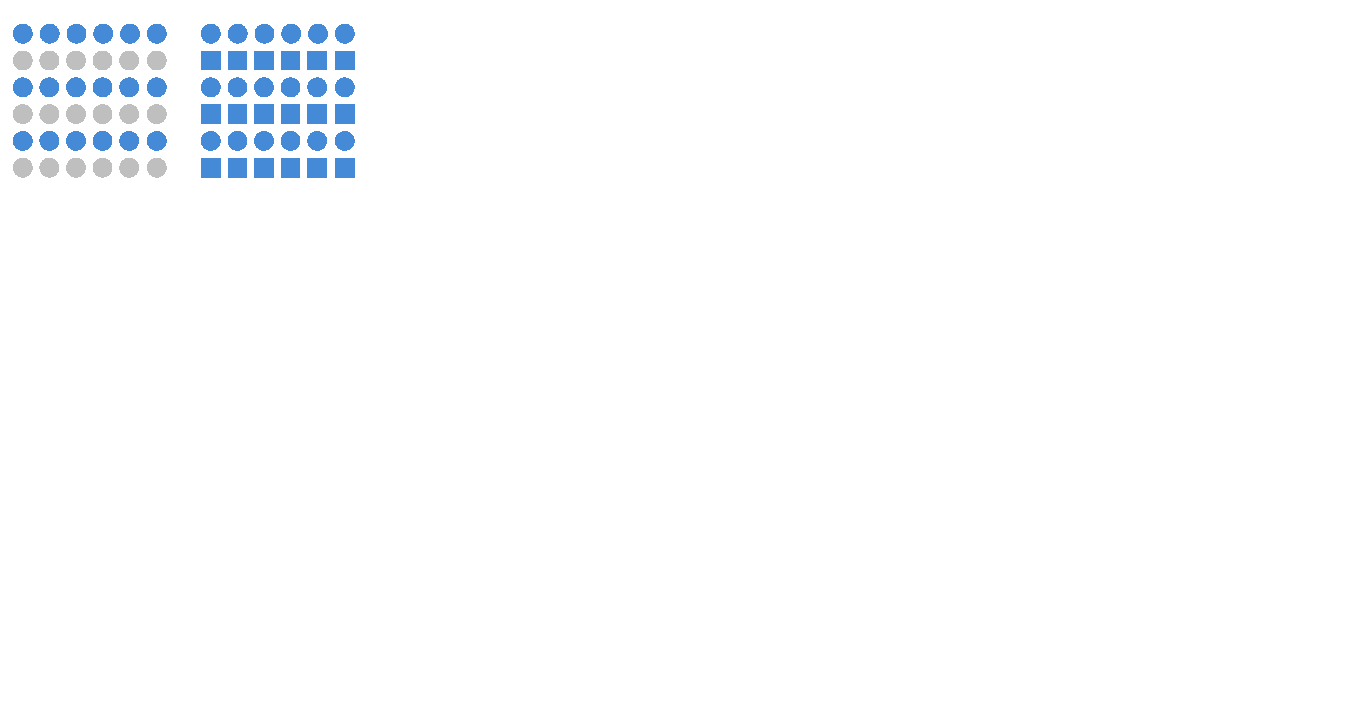
\includegraphics[width=1\textwidth]{gestalt-similarity}
\caption{\label{fig:simi} We perceive similar elements as a group \cite{Ware12}.}%[-1\baselineskip]
\end{marginfigure}

\textbf{Similarity} is the second Gestalt law. Visual similarities such as color or shape allow us to identify groups of objects with ease (cf. Fig.~\ref{fig:simi}). Large tables, for instance, can benefit from alternated shading of rows. A downside of shading is the additional visual clutter. We prefer to add additional space every three to five rows to keep tables readable. The similarity law is also important in diagrams that use different shapes or styles. Visual differences help the reader group similar elements.


\begin{marginfigure}
\centering
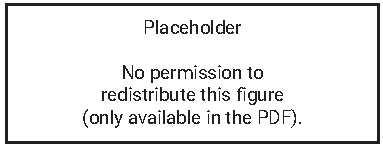
\includegraphics[width=1\textwidth]{gestalt-connectedness}
\caption{\label{fig:connectedness} Connections are more powerful than similarity \cite{Ware12}.}%[-1\baselineskip]
\end{marginfigure}

\textbf{Connectedness} is a powerful principle that is stronger than proximity, shape, and style.  (cf. Fig.~\ref{fig:connectedness}). Consider connecting related objects with lines.

The next principle, \textbf{continuity}, ``states that we are more likely to construct visual entities out of visual elements that are smooth and continuous, rather than ones that contain abrupt changes in direction.'' \cite{Ware12} It is, therefore, not surprising that node-link diagrams with smooth lines are easier to read than those with straight lines (cf. Fig.~\ref{fig:continuity}).

\begin{marginfigure}
\centering
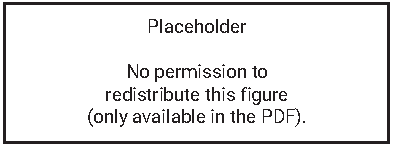
\includegraphics[width=1\textwidth]{gestalt-continuity}
\caption{\label{fig:continuity} Continuity makes the left-hand diagram easier to read \cite{Ware12}.}%[-1\baselineskip]
\end{marginfigure}

\begin{figure}
\centering
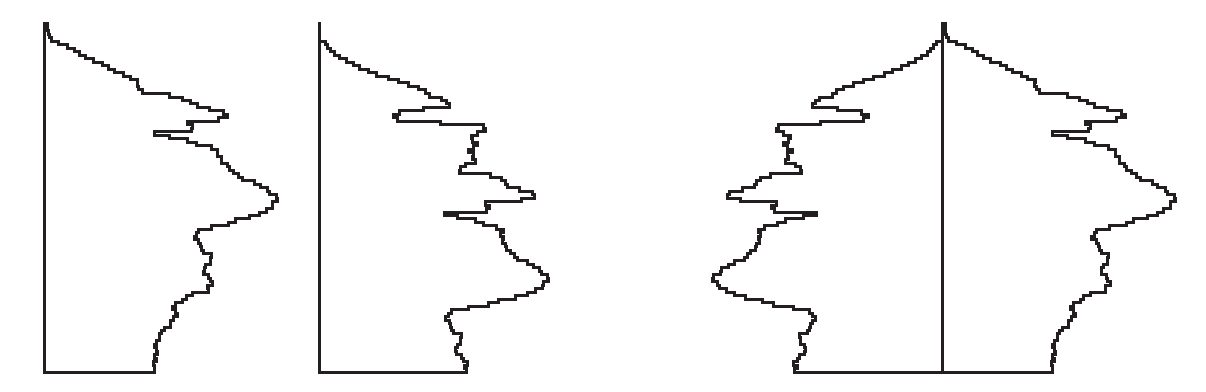
\includegraphics[width=1\textwidth]{gestalt-symmetry}
\sidecaption{\label{fig:symmetry} We can spot differences in these age distribution plots faster when data is plotted symmetrically (Data source: \url{https://destatis.de}).}[-4\baselineskip]
\end{figure}

Another principle is \textbf{symmetry}. Symmetrical figures are visually pleasing and we are good at detecting asymmetry. Symmetry is a form of high-level similarity. If you organize groups of elements in a diagram symmetrically, readers will assume that this means that they are similar. If you design diagrams asymmetrically, the asymmetric parts get emphasized. Our ability to check for symmetry can also be useful during visual data analysis (cf. Fig.~\ref{fig:symmetry}).

\begin{marginfigure}
\centering
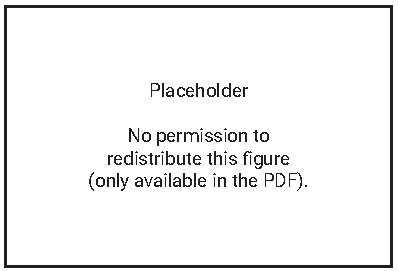
\includegraphics[width=1\textwidth]{gestalt-closure}
\caption{\label{fig:closure} Left: closure makes us perceive a full circle \cite{Ware12}; right: the orange dot is perceived to sit inside of a rectangle.}%[-1\baselineskip]
\end{marginfigure}

We are also on the lookout for \textbf{closure and common ground}. Closed contours are perceived as objects. Our search for closure is so strong that our brain interpolates missing parts of contours to form whole objects. This is why we see a rectangle and a complete circle on the left-hand side of Fig.~\ref{fig:closure} instead of a circle with a missing segment. Moreover, contours create a notion of a common ground with an ``inside'' and an ``outside''.

Common grounds are perceived for complete contours as well as for contours that we perceive due to closure. Thus, on the right-hand side of Fig.~\ref{fig:closure} we perceive the orange dot to be inside an imaginary rectangle built by shapes. Ware recommends: ``Consider putting related information inside a closed contour. A line is ade- quate for regions having a simple shape. Color or texture can be used to define regions that have more complex shapes.'' \cite{Ware12}.

The final Gestalt law to discuss is \textbf{figure and ground}. Figures are perceived as objects that are positioned in the foreground. The ground lies behind the figures. We perceive an object as a figure when it consists of a closed contour that forms a common ground and when it is considerably smaller in comparison to its surroundings.

\begin{marginfigure}
\centering
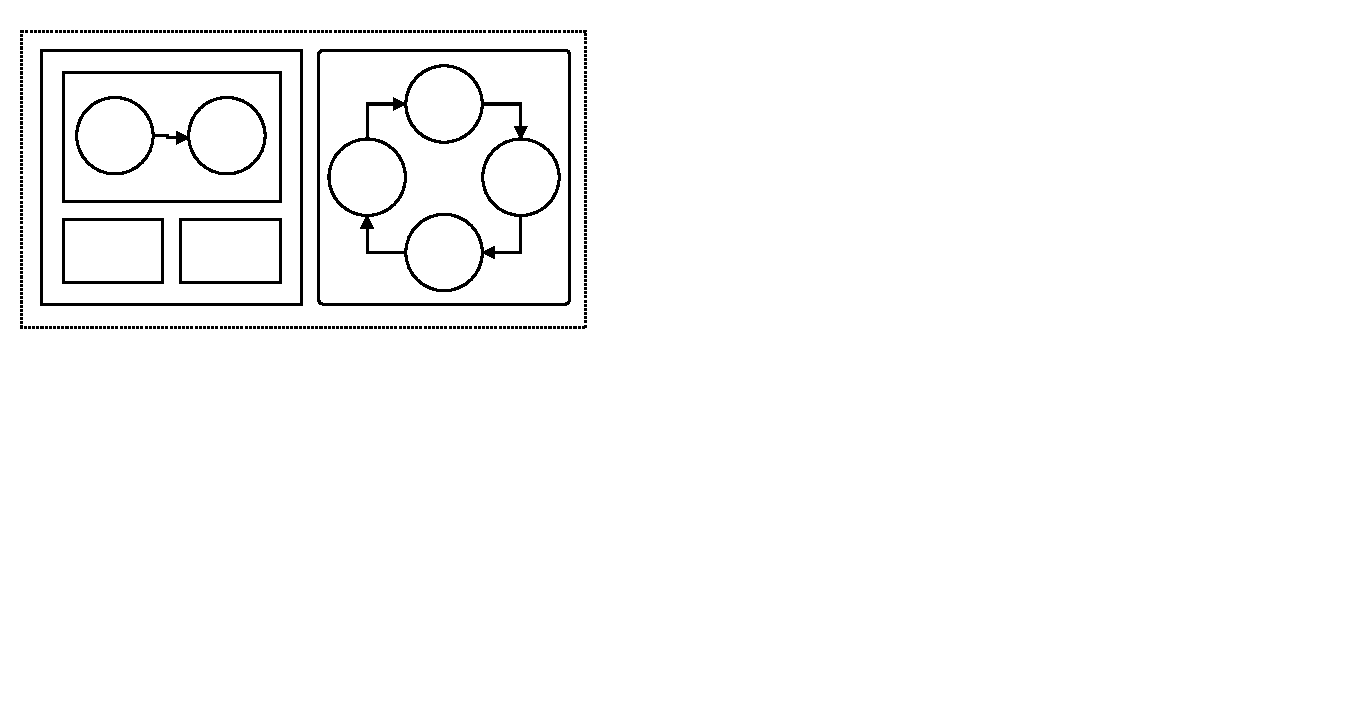
\includegraphics[width=1\textwidth]{gestalt-figureground}
\caption{\label{fig:figureground} Figure and ground are difficult to pick apart in this diagram (also note how PowerPoint fails to draw straight connectors).}%[-1\baselineskip]
\end{marginfigure}

This principle is important when drawing diagrams that use contours to demarcate the boundaries of various systems. When multiple systems are nested and the size differences are too small, it can become difficult to perceive the difference between figure and ground. Consider the diagram shown in Fig.~\ref{fig:figureground}). In the left-hand side of this diagram too many rectangular shapes have been nested. Due to equal amounts of whitespace around every shape, multiple interpretations are possible. The right-hand side of the diagram is slightly better because the circles are considerably smaller than the surrounding rectangle. Moreover, together with the arrows the circles are perceived as a (symmetric) shape, which is easily perceived as a figure sitting on the rectangle in the background.


% Gestalt Theory and Instructional Design , Moore and Fitz 1993
% http://citeseerx.ist.psu.edu/viewdoc/download?doi=10.1.1.1026.6390&rep=rep1&type=pdf


\subsection{Color}

You are probably used to defining colors in terms of red, green, and blue (RGB) or cyan, magenta, yellow, and black (CMYK). A third way, which is more useful, is the \textbf{HSB model}. It defines color in terms of hue, saturation, and brightness.\sidenote{Read the primer at \url{https://learnui.design/blog/the-hsb-color-system-practicioners-primer.html} for more details.} Consider the color picker shown in Fig.~\ref{fig:hsb} for an example.

\begin{figure}
\centering
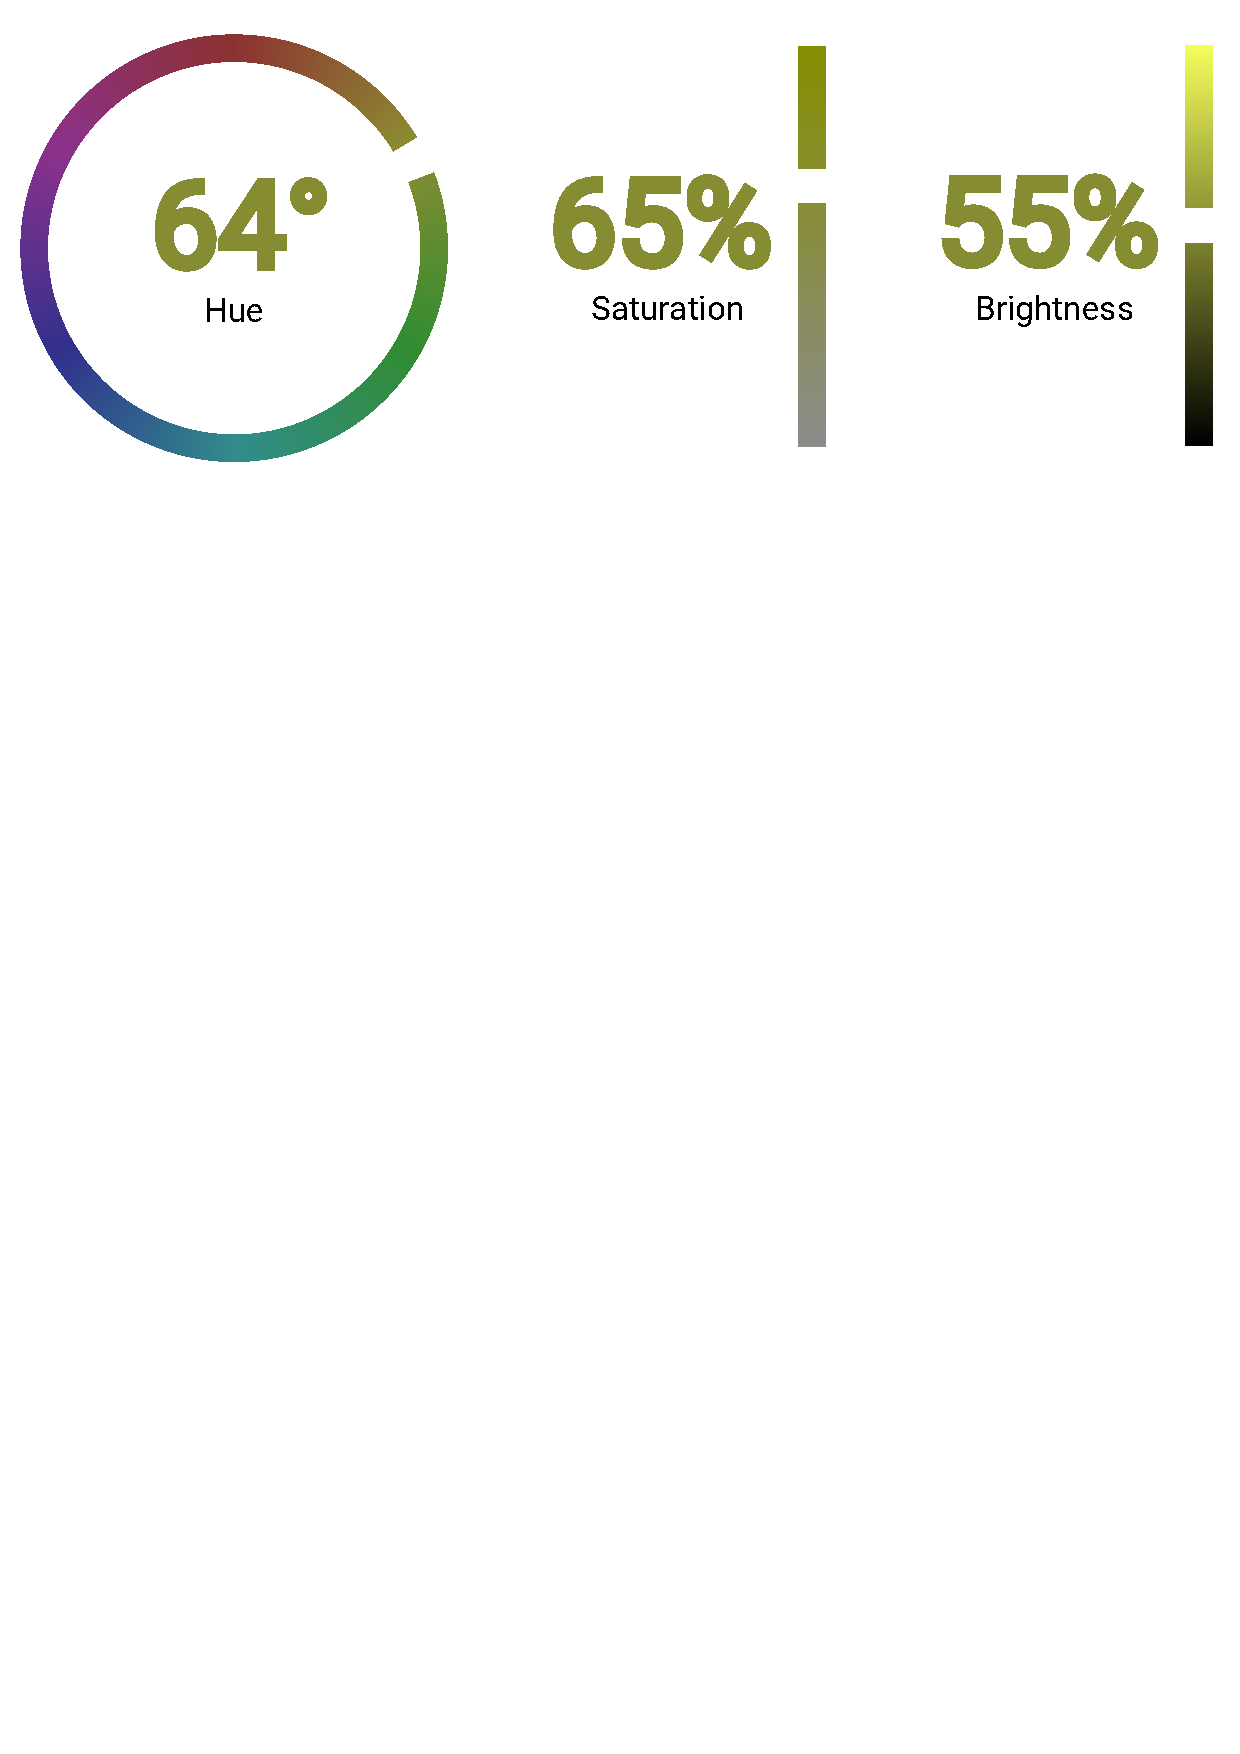
\includegraphics[width=0.85\textwidth]{color-hsb}
\sidecaption{\label{fig:hsb} A HSB color picker (\url{https://codepen.io/HunorMarton/full/eWvewo})}[-2\baselineskip]
\end{figure}

The first value, \textbf{hue}, defines the color according to its position (given in degrees ranging from 0 to 360) on the color wheel. For instance, the value 60 corresponds to the hue yellow. \textbf{Saturation} (0 to 100) corresponds to the richness of the color, where 0 means that there is no trace of the hue, i.\,e., a gray color between white and black. The value 100 means that the hue is fully present, i.\,e., the color is as colorful as possible. The final value is \textbf{brightness} (0 to 100). A value of 0 corresponds to a solid black (regardless of hue and saturation), a value of 100 corresponds to the brightest version of the hue at the given saturation.

Different colors are often used to ease visual perception (cf. Fig.~\ref{fig:coloredgraphs}). For instance, it can be used for emphasis, to group subsets of elements, or to make it easier to distinguish different elements that have a similar shape.

\begin{marginfigure}
\centering
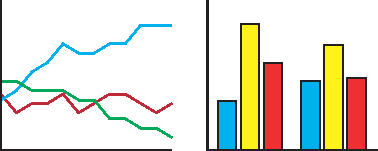
\includegraphics[width=1\textwidth]{color-plots}
\caption{\label{fig:coloredgraphs} Using colors to ease visual perception \cite{Carter12}.}%[-1\baselineskip]
\end{marginfigure}


Be aware of the monochrome representation of colors, which makes it impossible to distinguish a subset of colors. Red and green are particularly difficult to distinguish in monochrome print, especially if they have the same saturation and brightness (cf. Fig.~\ref{fig:monochrome}).

\begin{marginfigure}
\centering
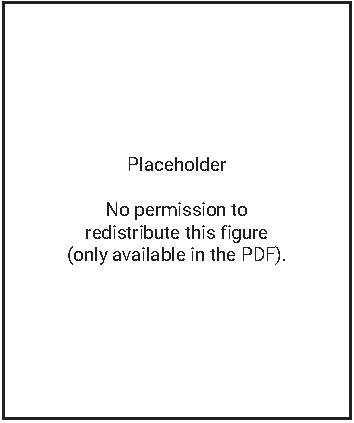
\includegraphics[width=0.8\textwidth]{color-mono}
\caption{\label{fig:monochrome} Colors in monochrome \cite{Carter12}.}%[-1\baselineskip]
\end{marginfigure}

The risk of confusion in monochrome prints is not the only reason why changing the hue is problematic. Different hues are difficult to make out when the area is small, as in the line plot in  Fig.~\ref{fig:coloredgraphs}. Moreover, different colors (hues) have different connotations (such as green means good, red means danger). Finally, different colors have different visual weight that may create unwanted emphasis (blue is heavier than orange).

Therefore, it is often better to stick with one hue and use different levels of brightness or saturation to ease visual perception. Figure~\ref{fig:monographs} uses three shades of gray and is easier to read than the colorful version in Fig.~\ref{fig:coloredgraphs}.


\begin{marginfigure}
\centering
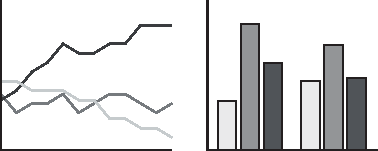
\includegraphics[width=1\textwidth]{color-plots-mono}
\caption{\label{fig:monographs} Shades of gray can be very effective \cite{Carter12}.}%[-1\baselineskip]
\end{marginfigure}

When you use more than four different grayscale colors, however, the differences become too small to perceive with ease. Too many grayscale colors are especially problematic when color is used on its own, such as in line plots. It is less problematic in bar plots, because the bars can be sorted with decreasing levels of brightness to create (good) redundancy. If brightness is used to encode values of data, darker color should be used for higher values.

Similar principles apply for saturation: ``If using color saturation to encode numerical quantity, use greater saturation to represent greater numerical quantities. Avoid using a saturation sequence to encode more than three values.'' \cite{Ware12} Consider varying both brightness and saturation at the same time to create shades that are easier to distinguish from another.

\begin{marginfigure}
\centering
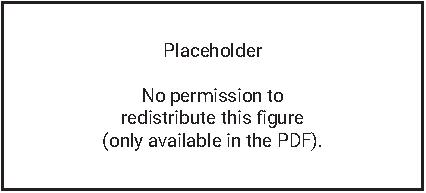
\includegraphics[width=1\textwidth]{color-saturation}
\caption{\label{fig:saturation} Use less saturation for large shapes, and more for thin lines \cite{Ware12}.}%[-2\baselineskip]
\end{marginfigure}

The effects of different levels of saturation vary depending on the size of the colored area (cf. Fig.~\ref{fig:saturation}). If you consider varying saturation, stick to the following guidelines: ``Use more saturated colors when color coding small symbols, thin lines, or other small areas. Use less saturated colors for coding large areas.'' \cite{Ware12}



\section{Diagrams}

You can use diagrams to describe concepts and their relationship, the structure of systems, interactions, and (experimental) procedures.

\subsection{Common Problems}

% infohq

% examples

\subsection{Before You Start}

Your first task is to decide \emph{whether a visualization makes sense at all}. Sometimes it makes sense to choose a text-only representation such as pseudo code instead of a diagram. Ware \cite{Ware12} shares the example of a flow chart, which is supposed to make it easier to understand the program flow (cf. Fig.~\ref{fig:flowchart}). He argues that pseudo code is superior. After all, the flow chart takes more effort to parse than the natural language used in the pseudo code (and, as Edward Tufte would argue, the flow chart contains more visual clutter than the pseudo code).

\begin{figure}[t]
\centering
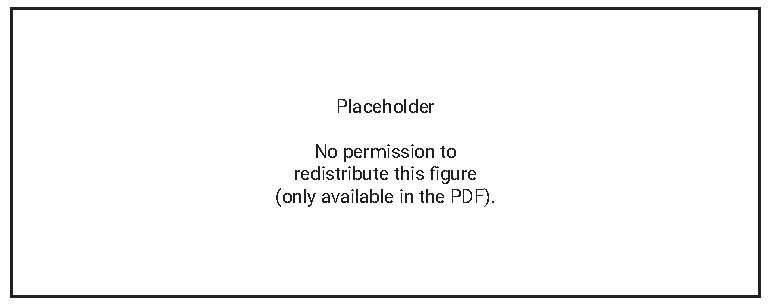
\includegraphics[width=1\textwidth]{diagram-flowchart}
\sidecaption{\label{fig:flowchart} According to Ware \cite{Ware12}, in comparison to pseudo code a flow chart is a poor representation of program flow.}[-4\baselineskip]
\end{figure}

On the other hand, Ware argues, there are concepts that we can grasp much faster if we see a visual representation. Consider the following statements about a management hierarchy \cite{Ware12}:

\begin{itemize}
  \item Jane is Jim’s boss.
  \item Jim is Joe’s boss.
  \item Anne works for Jane.
  \item Mark works for Jim.
  \item Anne is Mary’s boss.
  \item Anne is Mike’s boss
\end{itemize}


\begin{marginfigure}
\centering
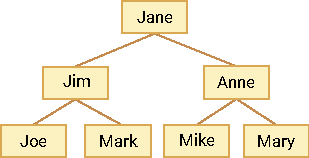
\includegraphics[width=1\textwidth]{diagram-tree}
\caption{\label{fig:tree} A tree helps us grasp static relationships \cite{Ware12}.}%[-2\baselineskip]
\end{marginfigure}

It is difficult to keep track of all relationships in this presentations. You might even feel the urge to draw a tree. And, indeed, a graphical representation is much more accessible (cf. Fig.~\ref{fig:tree}). Ware concludes: ``Diagrams should be used to express structural relationships among program elements, whereas words should be used to express detailed procedural logic'' \cite{Ware12}.


Now, if you decide that you do want to create a diagram, you should ask yourself the following questions \cite{Carter12}:
\begin{itemize}
\item What is absolutely necessary to show?
\item What is not necessary to show?
\item What is most important and should be emphasized?
\item What is not important and should be secondary to the main message?
\item What are the relationships between individual elements?
\item Does the diagram require a precise depiction of time?
\item Does the diagram require a precise depiction of distance?
\item What symbols should be consistent throughout the diagram?
\end{itemize}

In the following sections we will explain the most important aspects to create effective diagrams.

\subsection{Elements and Relationships}

According to the Gestalt laws, you should
``use small, closed shapes to represent data entities, and use the color, shape, and size of those shapes to represent attributes of those entities'' \cite{Ware12}. Figure~\ref{fig:entities} shows the effect of different properties of shapes.

\begin{figure}[t]
\centering
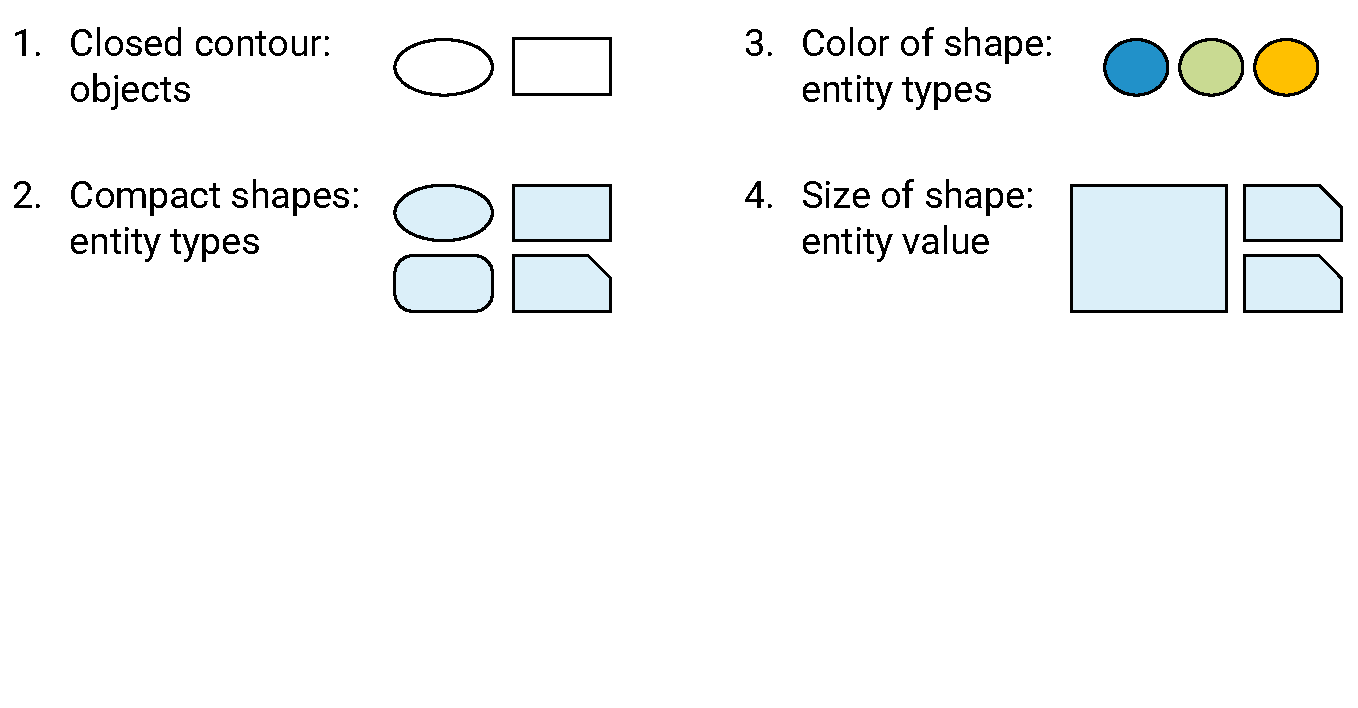
\includegraphics[width=1\textwidth]{diagram-entities}
\sidecaption{\label{fig:entities} Semantics of four properties of shapes \cite{Ware12}.}[-3\baselineskip]
\end{figure}

Many diagrams are supposed to visualize relationships of elements. Ware recommends to use ``connecting lines, enclosure, grouping, and attachment to represent relationships between entities. The shape, color, and thickness of lines and enclosures can represent the types of relationships'' \cite{Ware12}. Figure~\ref{fig:relationships} visualizes ten alternatives and how we perceive them.

Of note are the tapered lines in Number 6 of Fig.~\ref{fig:relationships}. As explained by Ware, these are easier to recognize than arrows \cite{Ware12}, especially in busy diagrams. If you only use straight lines, you can use very thin triangles to create tapered lines. The broad end is located at the source of the line.

For more complex lines, you will need a vector drawing tool like Inkscape, Adobe Illustrator, and Affinity Designer. Such tools will also allow you to draw the wiggly line shown in Number 7 of Fig.~\ref{fig:relationships}. In contrast, most drawing tools will allow you to create shapes with receptables (cf. Number 9 of Fig.~\ref{fig:relationships}) by creating unions and differences of shapes.



\begin{figure}[t]
\centering
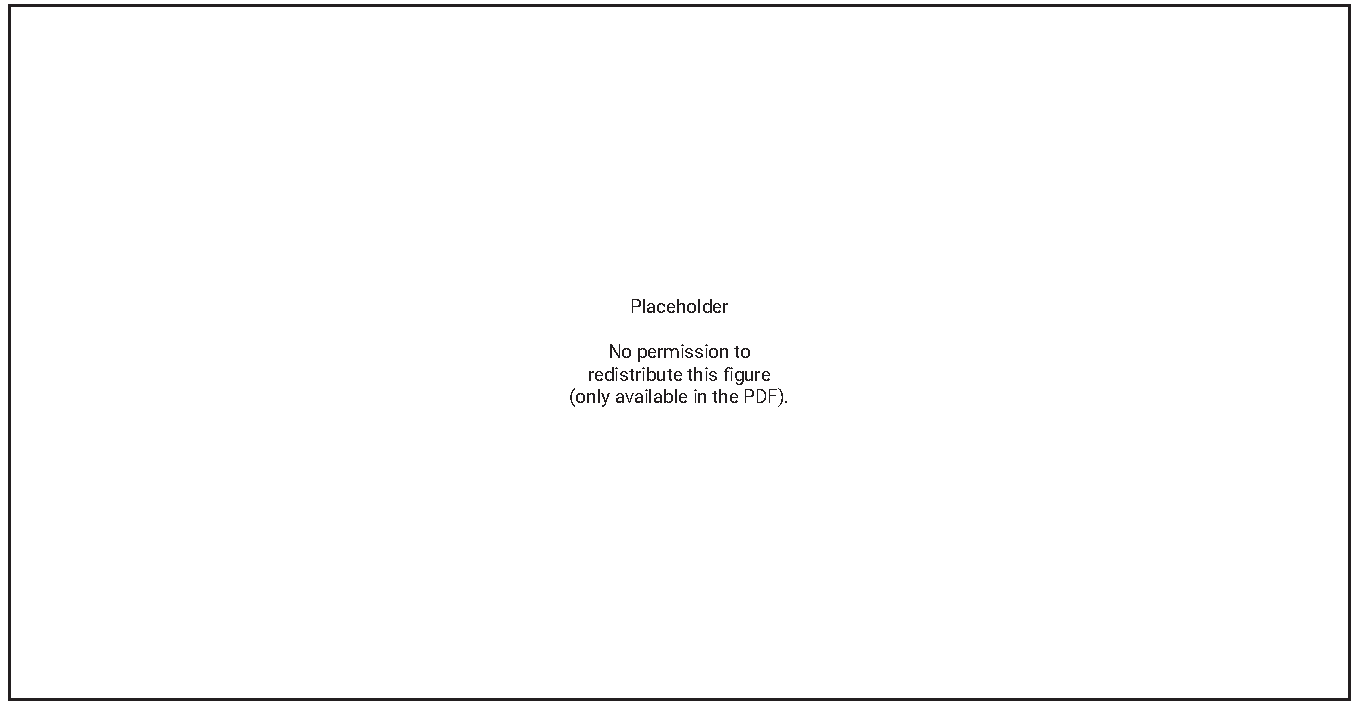
\includegraphics[width=1\textwidth]{diagram-relationships}
\sidecaption{\label{fig:relationships} Semantics of ten types of visual relationships \cite{Ware12}.}[-3\baselineskip]
\end{figure}



\subsection{Emphasizing Elements}

Good diagrams are self-explanatory and guide the reader's attention. Humans constantly search for patterns and deviations. Consistent use of shapes and colors indicates that the presented elements are similar (cf. Fig.~\ref{fig:emphasis}). Deviations from the norm indicate differences that need attention. Be aware of that and do not create emphasis unintentionally.

\begin{figure}[t]
\centering
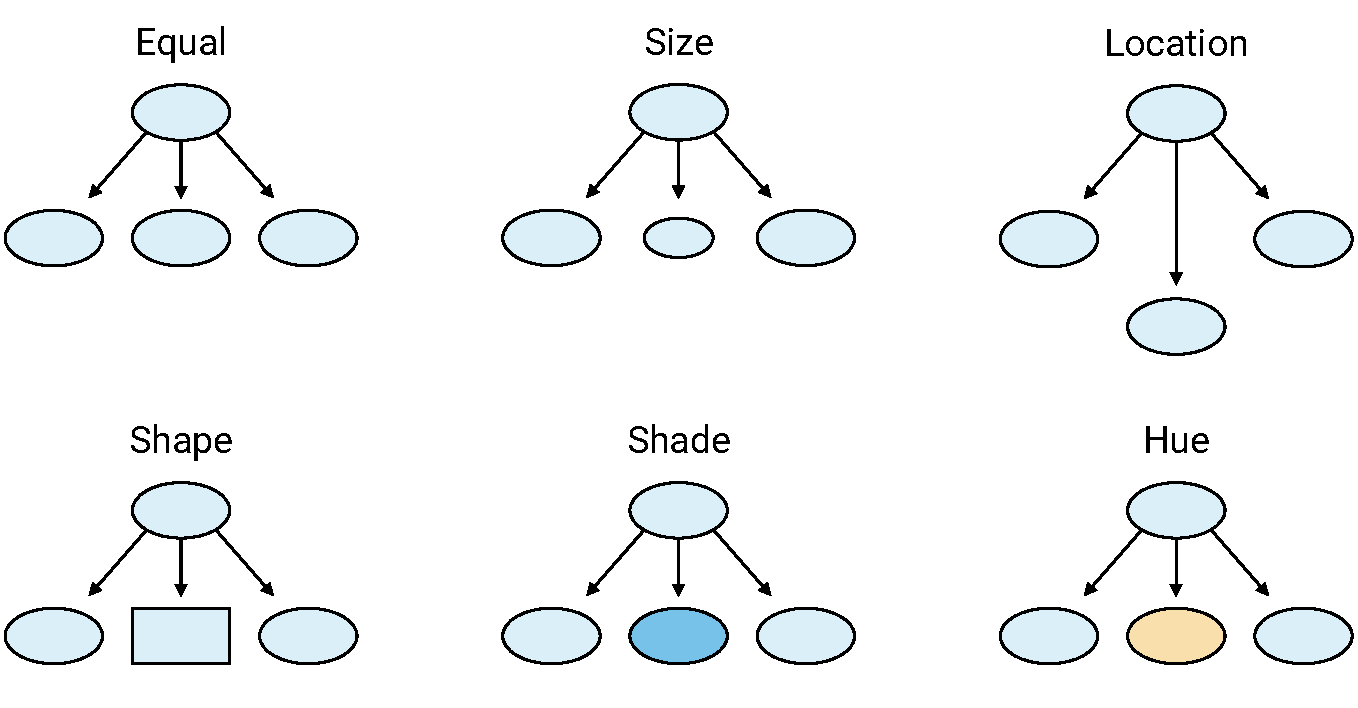
\includegraphics[width=1\textwidth]{diagram-emphasis}
\sidecaption{\label{fig:emphasis} Deviations from the norm create emphasis \cite{Carter12}.}[-4\baselineskip]
\end{figure}

Do not choose the size of elements arbitrarily. Differences translate into dominance relationships. Larger elements usually appear to control the smaller ones (cf. Fig.~\ref{fig:dominance})

\begin{figure}[t]
\centering
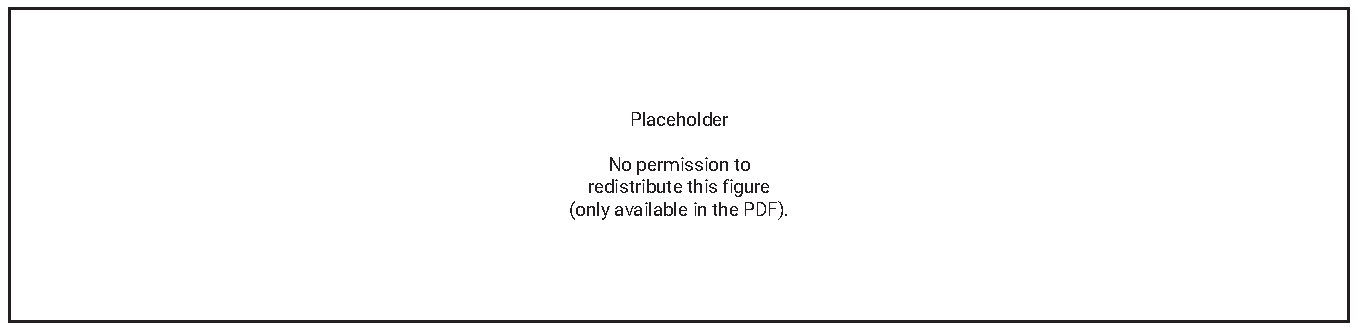
\includegraphics[width=1\textwidth]{diagram-dominance}
\sidecaption{\label{fig:dominance} Relative differences in size indicate dominance relationships \cite{Carter12}.}[-4\baselineskip]
\end{figure}


\subsection{Layout}

In the absence of strong emphasis, readers process diagrams similar to text (cf. Fig.~\ref{fig:direction}). In western cultures, readers will start in the top left corner and proceed horizontally in a zig-zag pattern. The general flow of information should be consistent with this expectation.

\begin{marginfigure}
\centering
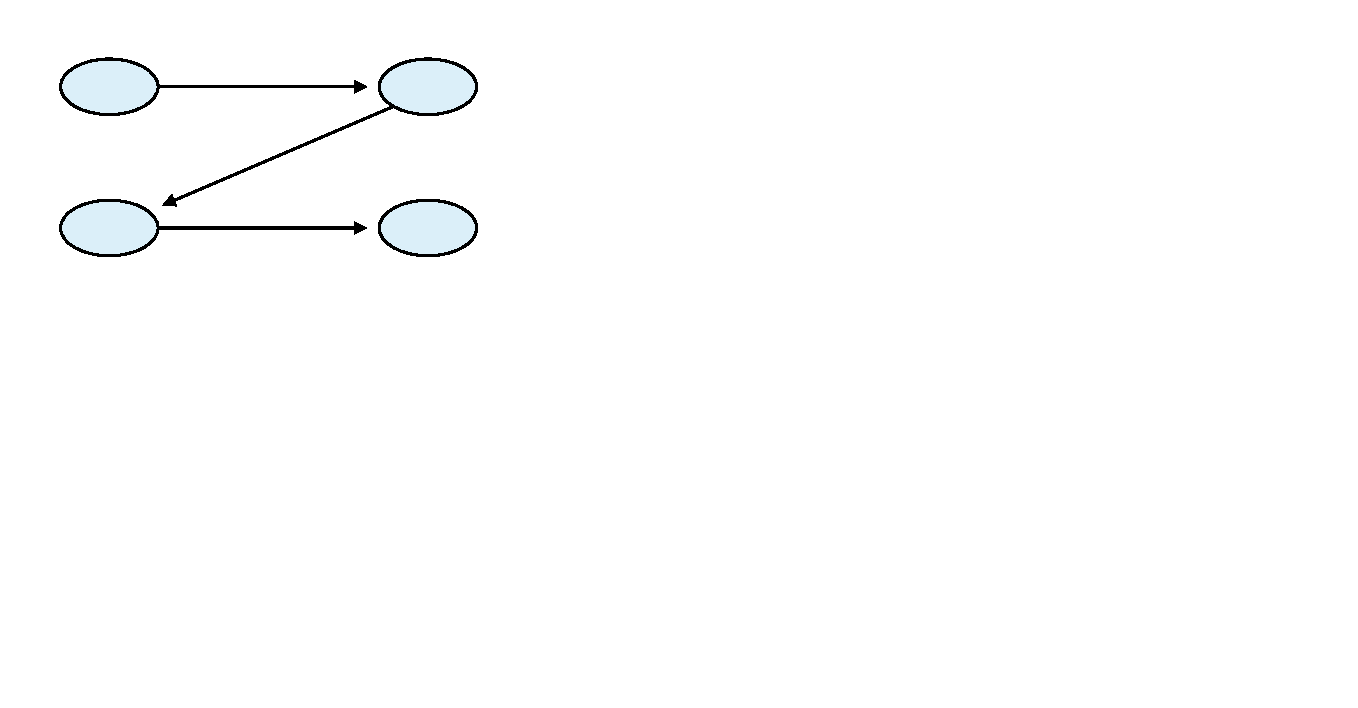
\includegraphics[width=1\textwidth]{diagram-direction}
\caption{\label{fig:direction} Respect the expected flow of information in western cultures \cite{Carter12}.}%[-1\baselineskip]
\end{marginfigure}


Ensure that all elements of a diagram are properly aligned. Alignment helps readers to grasp the overall structure. Proper alignment can also save you from creating additional outlines to depict (systems) boundaries – proximity and neat alignment can create strong cohesion by themselves (closure).

Make conscious decisions about distances and dimensions (proximity, repetition). You \emph{can} use a \emph{grid} to enforce consistent distances. Note, however, that snapping every element to the grid lines, may still cause mis-alignment in some cases.\sidenote{Consider a shape that is four grid lines high. Then, a horizontal line that leaves the box cannot be aligned in the middle.} Make use of the horizontal and vertical alignment tools that space out elements equally. An advanced technique is to create a dummy box shape to measure and compare dimensions yourself.

\subsection{Labels}

Many diagrams consist of shapes and lines, annotated with text labels.

A commonplace technique is to use bold print to express some property of an element. For instance, the labels of all shapes that correspond to systems are printed in bold to differentiate these shapes from the ones that correspond to exchanged  messages. In general, we recommend to avoid this practice. Reserve bold print for emphasizing \emph{one particular element} in a diagram. Use another visual style to show differences, such as shading, colors, or shape form. Also consider the option of giving an element no surrounding shape at all, for instance, if the notion of its \emph{boundary} is not relevant or if the arrangement of sub-elements establishes a common ground due to the Gestalt law of \emph{closure}.

In any case, the labels should be as close as possible to the shapes (Gestalt law proximity) and exactly aligned. Whenever possible, consider moving the labels into the shapes (Fig.~\ref{fig:labelsinside}). Inside labels rely on the Gestalt law of \emph{common ground}. They reduce visual clutter and make it easier to create a well-balanced diagram that has no ragged edges (laws of symmetry and closure). 

\begin{figure}[t]
\centering
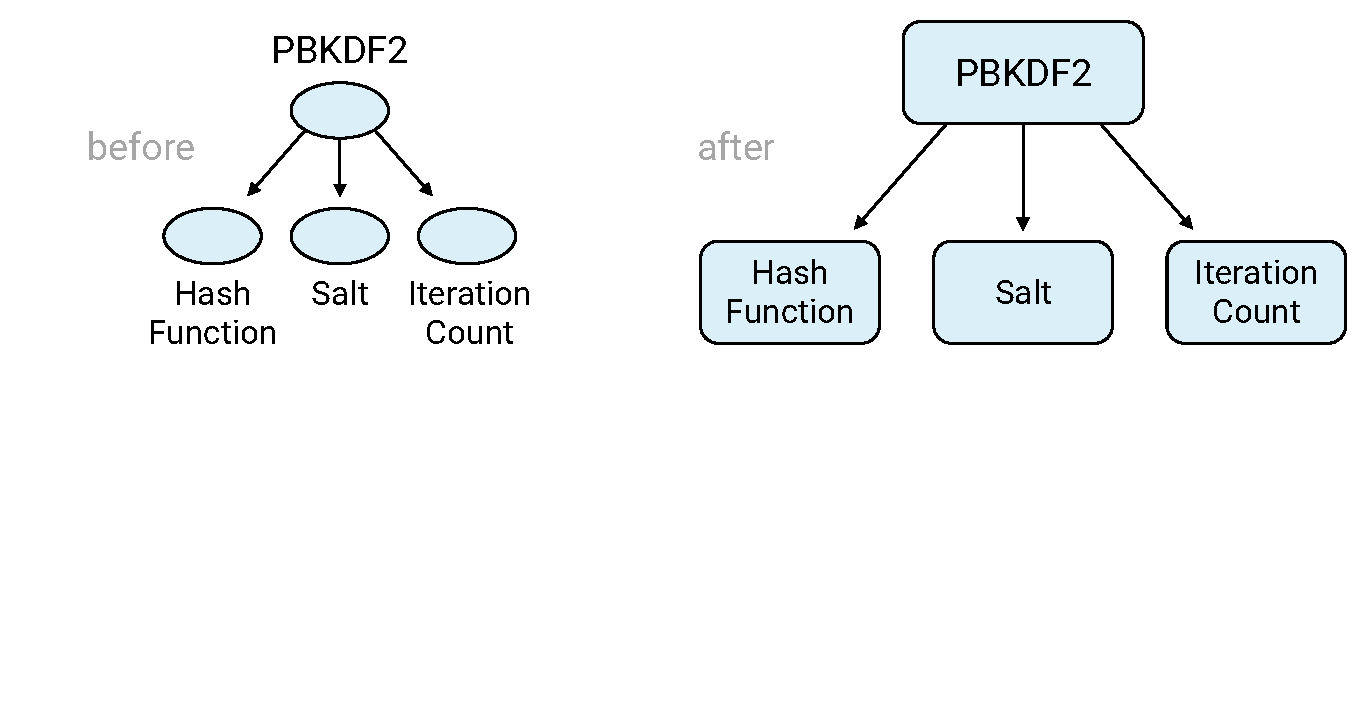
\includegraphics[width=1\textwidth]{diagram-labelsinside}
\sidecaption{\label{fig:labelsinside} Moving the labels inside objects reduces clutter. Note how the left-hand-side figure is centered in the left part of the figure to keep the figure balanced \cite{Carter12}.}[-6\baselineskip]
\end{figure}

\begin{marginfigure}
\centering
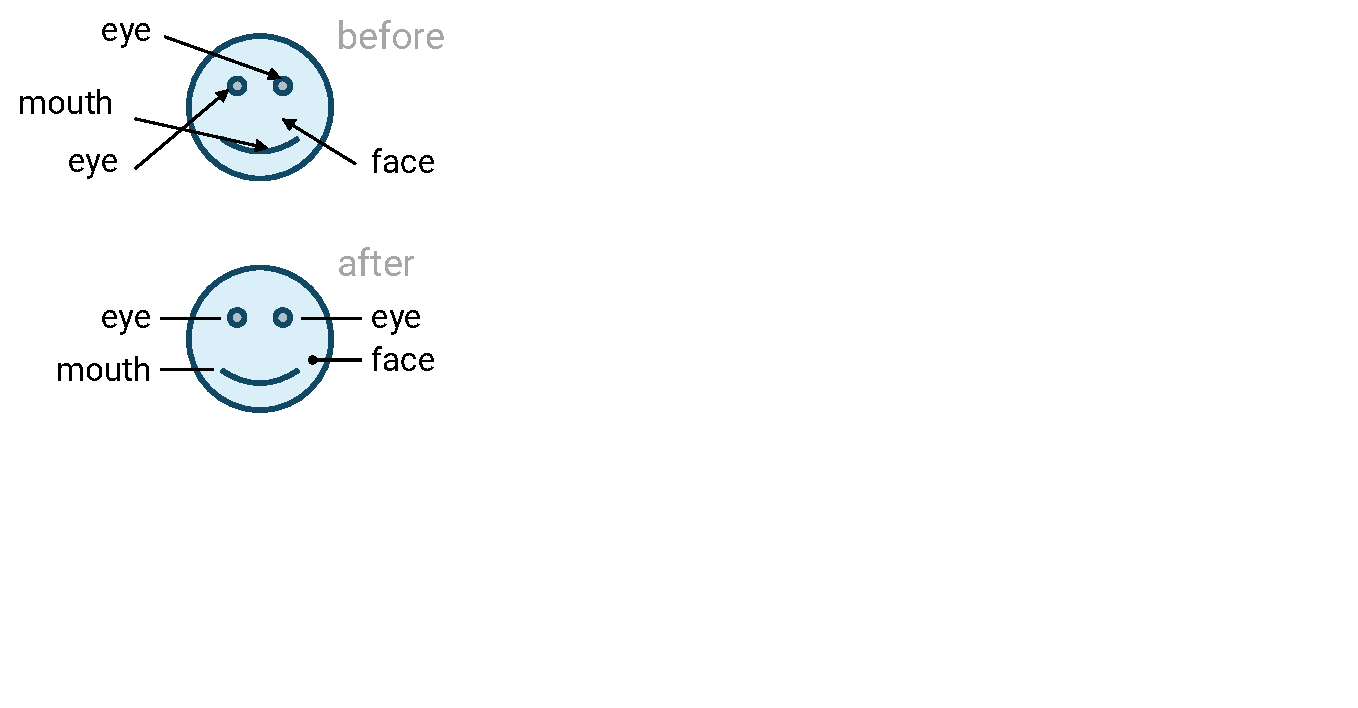
\includegraphics[width=1\textwidth]{diagram-labelsoutside}
\caption{\label{fig:labelsoutside} Outside labels should not distract the reader \cite{Carter12}.}%[-1\baselineskip]
\end{marginfigure}

Figure~\ref{fig:labelsoutside} illustrates key principles when labels are outside of a shape. First of all, keep the lines as short as possible (proximity). Consider removing the arrowheads from the lines that point into an object to avoid confusion with other arrows in the diagram. Also, avoid crossing lines. Align labels on the left-hand side of an object flush right and vice versa (symmetry). Aim for consistency by making the lines parallel. Keep adequate amounts of surrounding whitespace.

Diagrams that visualize structures can work fine with few labels. In contrast, diagrams that visualize procedures or more complex relationships need more textual explanation. Consider adding longer explanations right next to the corresponding locations (proximity) as shown in Fig.~\ref{fig:explanations}.

\begin{figure}[t]
\centering

\includegraphics[width=1\textwidth]{diagram-explanations} 
\sidecaption{\label{fig:explanations} Complex diagrams benefit from integrated explanations. Source of figure as cited by \cite{Ware12}: R Chandler and J. Sweller (1991). Cognitive load theory and the format of instruction. \emph{Cognition and Instruction, 8,} 293–332.}[-7\baselineskip]
\end{figure}


\subsection{Variations}

\begin{figure*}[t]
\centering
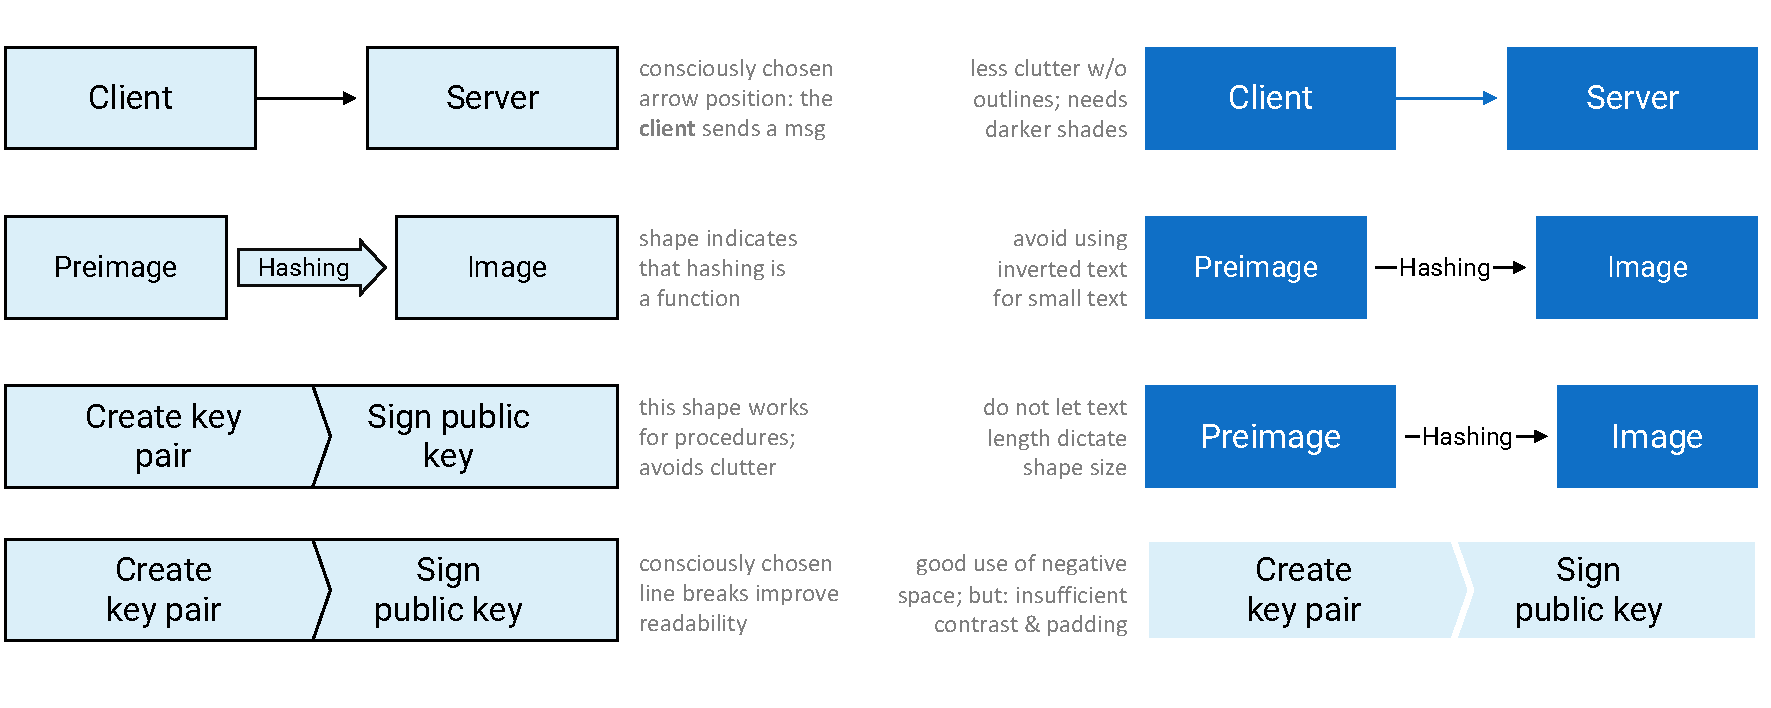
\includegraphics[width=1\widefigurewidth]{diagram-variations}
\sidecaption{\label{fig:diagvariations} Eight variations resulting from combining different outline, shade, and arrow styles.}[-1\baselineskip]
\end{figure*}

Common drawing tools provide a large number of shapes. What is missing, however, is guidance on how to combine them reasonably. Figure~\ref{fig:diagvariations} displays eight combinations.\sidenote{The advice in the following paragraphs has been compiled from \url{https://www.slideshare.net/otikik/how-to-make-awesome-diagrams-for-your-slides/19-Size_doesnt_mean_long_name}}

The first variation in the left-hand column shows a style useful for depicting information exchange between systems, such as servers and clients. The second variation uses an arrow shape. This emphasizes that the arrow corresponds to an activity itself. The third and fourth examples in the left-hand column depict two steps from a process without too much visual clutter. We prefer the latter one because the text wraps at sensible points.

The right-hand column shows variations without outlines. At first glance, this sounds like a good  idea: after all, it avoids visual clutter (the outlines). Note, however, that shapes without outlines need more saturated and darker color to differentiate them from the background.  If the number of shapes in a diagram is large, this approach can actually make it more difficult to read the diagram because all shapes appear to be emphasized at the same time.

If you use dark-colored shapes, you should avoid having white text on dark background for small font sizes. As shown in the second variation on the right-hand side of Fig.~\ref{fig:diagvariations}, you will have to make changes to some shapes.

In any case, you should choose the sizes of shapes consciously. Represent objects with identical properties with shapes of the same size. If the labels do not fit into the shapes, you can either reduce the font size, put the labels next to the box, or increase the size of all shapes (by rearranging the diagram).

Finally, consider the option of using negative space, as shown in the bottom-right corner of the Fig.~\ref{fig:diagvariations}. Again, this can be a useful means to avoid visual clutter. However, if you just increase the stroke width (as was done for the example figure), the (vertical) padding in the shape will become too narrow. Moreover, you cannot easily align such shapes with other shapes with thinner strokes.

\section{Figures}

















